
\documentclass[a4paper, 12pt, fleqn]{scrartcl}

\usepackage{math-practice}
\usepackage{circuitikz}

\area{TODO}
\title{Differenciálegyenletek}
\subject{Matematika G3}
\subjectCode{BMETE94BG03}
\date{Utoljára frissítve: \today}
\docno{10}

\begin{document}
\maketitle

\subsection{Elméleti Áttekintő}

\clearpage
\subsection{Feladatok}

\begin{enumerate}
  \item Egy soros RL-körre konstans $u_0$ feszültséget kapcsolunk. Adja meg
        az áram időfüggvényét!

        \begin{minipage}{.25\textwidth}
          \centering
          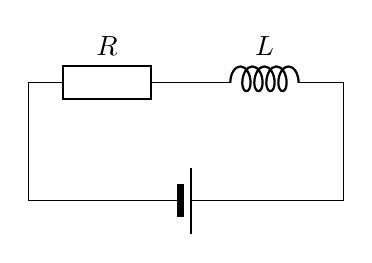
\begin{tikzpicture}[european resistors]
            \draw
            % (1.5,0) to[short,o-]
            (0,0)
            to (0,1.5)
            to[R=$R$] (2,1.5)
            to[L=$L$] (4,1.5)
            to (4,0)
            % to[short,-o] (2.5,0)
            to[battery2] (0,0)
            -- cycle
            ;
          \end{tikzpicture}
        \end{minipage}\begin{minipage}{.4\textwidth}
          \begin{align*}
            u_R & = R \cdot i
            \\
            u_L & = L \cdot \odv{i}{t}
          \end{align*}
        \end{minipage}

  \item TODO lánc

  \item Oldja meg az alábbi egzakt, illetve egyakttá tehető
        differenciálegyenleteket!
        \begin{enumerate}
          \item $\displaystyle
                  (2x + 2 \sin y) \dd x
                  + (2x \cos y - \sin y) \dd y
                  = 0
                $,
                \vspace{2mm}

          \item $\displaystyle
                  (1 - xy) \dd x
                  + (xy - x^2) \dd y
                  = 0
                $,

          \item $\displaystyle
                  \left( \ln (y^2 + 1) \right) \dd x
                  + \frac{2y(x - 1)}{y^2 + 1} \dd y
                  = 0
                $,

          \item $\displaystyle
                  e^{-y} \dd x
                  + \left( x \, e^{-y} - 2y \, e^{-2y} \right) \dd y
                  = 0
                $.
        \end{enumerate}

  \item Oldja meg az alábbi Bernoulli-féle differenciálegyenletet!
        $$
          y' - \frac{3y}{x} = x^4 y^{1/3}
        $$

  \item Oldja meg az alábbi Ricatti féle differenciálegyenletet!
        $$
          y' = xy^2 - (4 - 2x^2)y + x^3 + 4x + 1
        $$
\end{enumerate}
\end{document}